% This file is generated by the MATLAB m-file laprint.m. It can be included
% into LaTeX documents using the packages graphicx, color and psfrag.
% It is accompanied by a postscript file. A sample LaTeX file is:
%    \documentclass{article}\usepackage{graphicx,color,psfrag}
%    \begin{document}% This file is generated by the MATLAB m-file laprint.m. It can be included
% into LaTeX documents using the packages graphicx, color and psfrag.
% It is accompanied by a postscript file. A sample LaTeX file is:
%    \documentclass{article}\usepackage{graphicx,color,psfrag}
%    \begin{document}% This file is generated by the MATLAB m-file laprint.m. It can be included
% into LaTeX documents using the packages graphicx, color and psfrag.
% It is accompanied by a postscript file. A sample LaTeX file is:
%    \documentclass{article}\usepackage{graphicx,color,psfrag}
%    \begin{document}% This file is generated by the MATLAB m-file laprint.m. It can be included
% into LaTeX documents using the packages graphicx, color and psfrag.
% It is accompanied by a postscript file. A sample LaTeX file is:
%    \documentclass{article}\usepackage{graphicx,color,psfrag}
%    \begin{document}\input{fig_4_5_tex}\end{document}
% See http://www.mathworks.de/matlabcentral/fileexchange/loadFile.do?objectId=4638
% for recent versions of laprint.m.
%
% created by:           LaPrint version 3.16 (13.9.2004)
% created on:           11-Jul-2009 20:12:04
% eps bounding box:     15 cm x 11.25 cm
% comment:              
%
\begin{psfrags}%
\psfragscanon%
%
% text strings:
\psfrag{s01}[t][t]{\color[rgb]{0,0,0}\setlength{\tabcolsep}{0pt}\begin{tabular}{c}$x_1$\end{tabular}}%
\psfrag{s02}[b][b]{\color[rgb]{0,0,0}\setlength{\tabcolsep}{0pt}\begin{tabular}{c}$x_2$\end{tabular}}%
%
% xticklabels:
\psfrag{x01}[t][t]{-10}%
\psfrag{x02}[t][t]{-5}%
\psfrag{x03}[t][t]{0}%
\psfrag{x04}[t][t]{5}%
\psfrag{x05}[t][t]{10}%
%
% yticklabels:
\psfrag{v01}[r][r]{-10}%
\psfrag{v02}[r][r]{-8}%
\psfrag{v03}[r][r]{-6}%
\psfrag{v04}[r][r]{-4}%
\psfrag{v05}[r][r]{-2}%
\psfrag{v06}[r][r]{0}%
\psfrag{v07}[r][r]{2}%
\psfrag{v08}[r][r]{4}%
\psfrag{v09}[r][r]{6}%
\psfrag{v10}[r][r]{8}%
\psfrag{v11}[r][r]{10}%
%
% Figure:
\resizebox{12cm}{!}{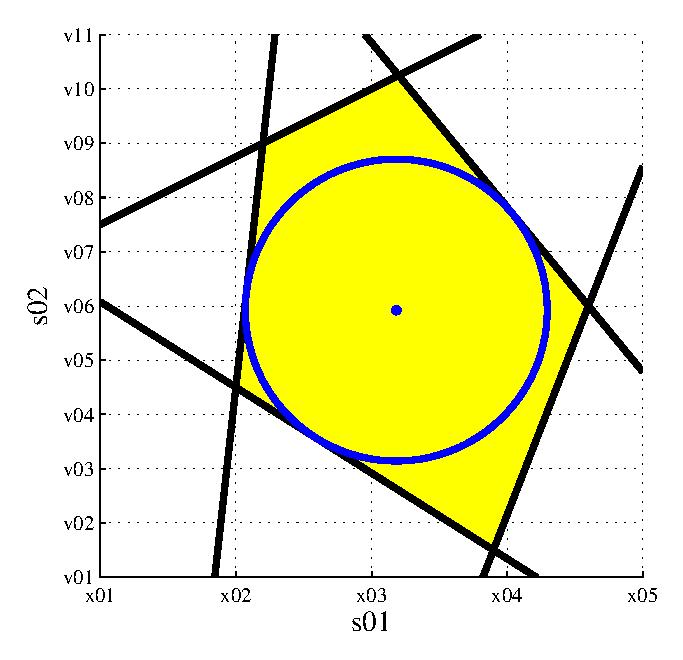
\includegraphics{fig_4_5_tex.eps}}%
\end{psfrags}%
%
% End fig_4_5_tex.tex
\end{document}
% See http://www.mathworks.de/matlabcentral/fileexchange/loadFile.do?objectId=4638
% for recent versions of laprint.m.
%
% created by:           LaPrint version 3.16 (13.9.2004)
% created on:           11-Jul-2009 20:12:04
% eps bounding box:     15 cm x 11.25 cm
% comment:              
%
\begin{psfrags}%
\psfragscanon%
%
% text strings:
\psfrag{s01}[t][t]{\color[rgb]{0,0,0}\setlength{\tabcolsep}{0pt}\begin{tabular}{c}$x_1$\end{tabular}}%
\psfrag{s02}[b][b]{\color[rgb]{0,0,0}\setlength{\tabcolsep}{0pt}\begin{tabular}{c}$x_2$\end{tabular}}%
%
% xticklabels:
\psfrag{x01}[t][t]{-10}%
\psfrag{x02}[t][t]{-5}%
\psfrag{x03}[t][t]{0}%
\psfrag{x04}[t][t]{5}%
\psfrag{x05}[t][t]{10}%
%
% yticklabels:
\psfrag{v01}[r][r]{-10}%
\psfrag{v02}[r][r]{-8}%
\psfrag{v03}[r][r]{-6}%
\psfrag{v04}[r][r]{-4}%
\psfrag{v05}[r][r]{-2}%
\psfrag{v06}[r][r]{0}%
\psfrag{v07}[r][r]{2}%
\psfrag{v08}[r][r]{4}%
\psfrag{v09}[r][r]{6}%
\psfrag{v10}[r][r]{8}%
\psfrag{v11}[r][r]{10}%
%
% Figure:
\resizebox{12cm}{!}{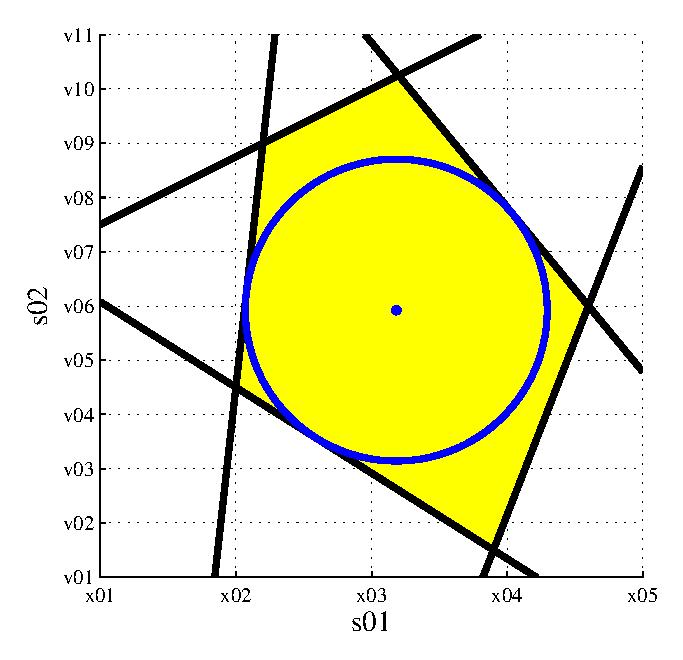
\includegraphics{fig_4_5_tex.eps}}%
\end{psfrags}%
%
% End fig_4_5_tex.tex
\end{document}
% See http://www.mathworks.de/matlabcentral/fileexchange/loadFile.do?objectId=4638
% for recent versions of laprint.m.
%
% created by:           LaPrint version 3.16 (13.9.2004)
% created on:           11-Jul-2009 20:12:04
% eps bounding box:     15 cm x 11.25 cm
% comment:              
%
\begin{psfrags}%
\psfragscanon%
%
% text strings:
\psfrag{s01}[t][t]{\color[rgb]{0,0,0}\setlength{\tabcolsep}{0pt}\begin{tabular}{c}$x_1$\end{tabular}}%
\psfrag{s02}[b][b]{\color[rgb]{0,0,0}\setlength{\tabcolsep}{0pt}\begin{tabular}{c}$x_2$\end{tabular}}%
%
% xticklabels:
\psfrag{x01}[t][t]{-10}%
\psfrag{x02}[t][t]{-5}%
\psfrag{x03}[t][t]{0}%
\psfrag{x04}[t][t]{5}%
\psfrag{x05}[t][t]{10}%
%
% yticklabels:
\psfrag{v01}[r][r]{-10}%
\psfrag{v02}[r][r]{-8}%
\psfrag{v03}[r][r]{-6}%
\psfrag{v04}[r][r]{-4}%
\psfrag{v05}[r][r]{-2}%
\psfrag{v06}[r][r]{0}%
\psfrag{v07}[r][r]{2}%
\psfrag{v08}[r][r]{4}%
\psfrag{v09}[r][r]{6}%
\psfrag{v10}[r][r]{8}%
\psfrag{v11}[r][r]{10}%
%
% Figure:
\resizebox{12cm}{!}{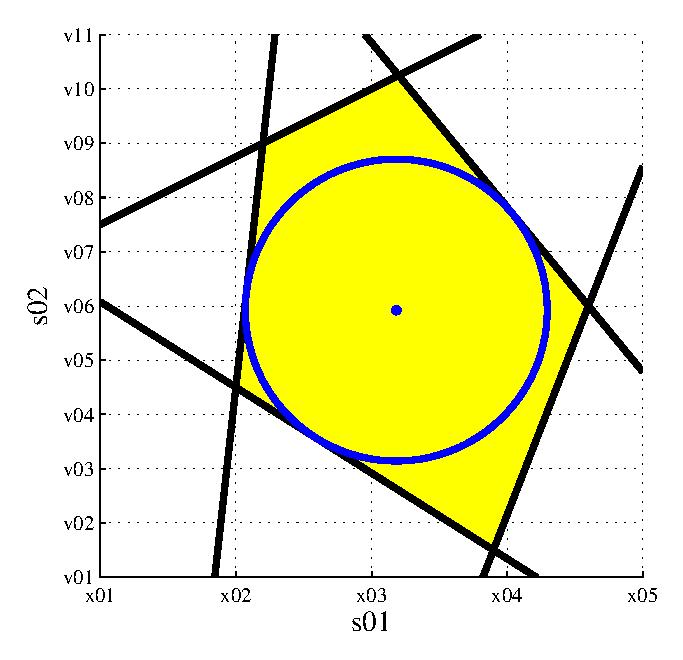
\includegraphics{fig_4_5_tex.eps}}%
\end{psfrags}%
%
% End fig_4_5_tex.tex
\end{document}
% See http://www.mathworks.de/matlabcentral/fileexchange/loadFile.do?objectId=4638
% for recent versions of laprint.m.
%
% created by:           LaPrint version 3.16 (13.9.2004)
% created on:           11-Jul-2009 20:12:04
% eps bounding box:     15 cm x 11.25 cm
% comment:              
%
\begin{psfrags}%
\psfragscanon%
%
% text strings:
\psfrag{s01}[t][t]{\color[rgb]{0,0,0}\setlength{\tabcolsep}{0pt}\begin{tabular}{c}$x_1$\end{tabular}}%
\psfrag{s02}[b][b]{\color[rgb]{0,0,0}\setlength{\tabcolsep}{0pt}\begin{tabular}{c}$x_2$\end{tabular}}%
%
% xticklabels:
\psfrag{x01}[t][t]{-10}%
\psfrag{x02}[t][t]{-5}%
\psfrag{x03}[t][t]{0}%
\psfrag{x04}[t][t]{5}%
\psfrag{x05}[t][t]{10}%
%
% yticklabels:
\psfrag{v01}[r][r]{-10}%
\psfrag{v02}[r][r]{-8}%
\psfrag{v03}[r][r]{-6}%
\psfrag{v04}[r][r]{-4}%
\psfrag{v05}[r][r]{-2}%
\psfrag{v06}[r][r]{0}%
\psfrag{v07}[r][r]{2}%
\psfrag{v08}[r][r]{4}%
\psfrag{v09}[r][r]{6}%
\psfrag{v10}[r][r]{8}%
\psfrag{v11}[r][r]{10}%
%
% Figure:
\resizebox{12cm}{!}{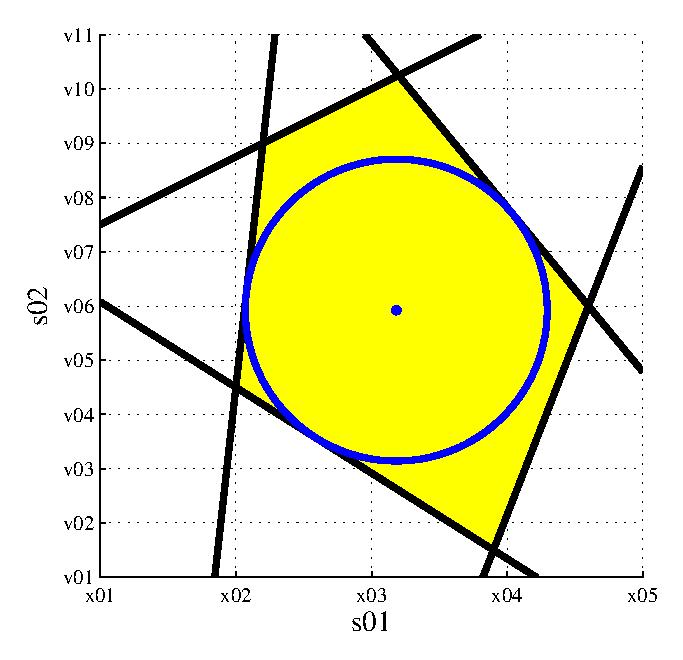
\includegraphics{fig_4_5_tex.eps}}%
\end{psfrags}%
%
% End fig_4_5_tex.tex
